\chapter{Gráficas de eficiencia clúster universitario \label{apenEficiencia}}
\section{Procesamiento de datos}
\begin{figure}[htp!]
	\centering
	\caption{Gráfica comparativa de la eficiencia en el procesamiento de los datos por el clúster universitario.}
	\label{gra:efiProcUniApen}
	\vspace{5pt}
	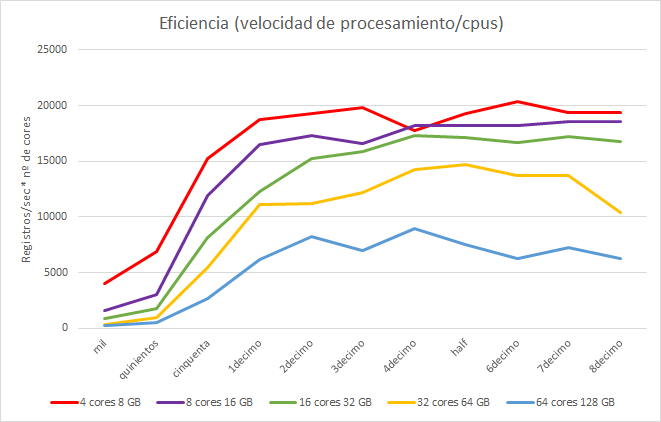
\includegraphics[scale=0.9]{graficas/epuni}
\end{figure}
\section{Rutas más frecuentes}
\begin{figure}[htp!]
	\centering
	\caption{Gráfica comparativa de la eficiencia durante la consulta de rutas frecuentes por el clúster universitario.}
	\label{gra:efiFreqUniApen}
	\vspace{5pt}
	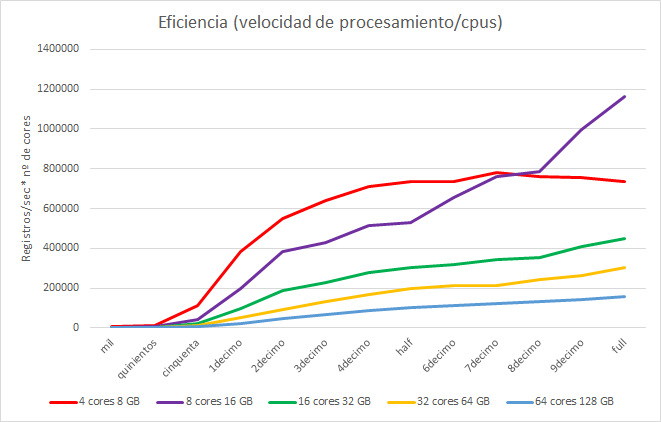
\includegraphics[scale=0.8]{graficas/efuni}
\end{figure}
\begin{figure}[htp!]
	\centering
	\caption{Gráfica comparativa de la eficiencia durante la consulta de rutas frecuentes teniendo en cuenta la estacionalidad por el clúster universitario.}
	\label{gra:efiFreqDayUniApen}
	\vspace{5pt}
	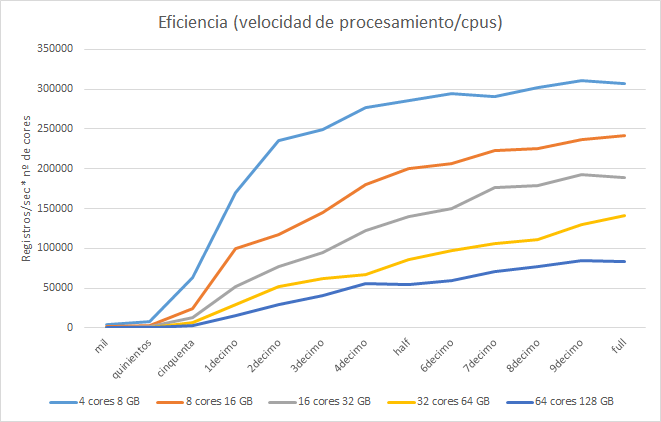
\includegraphics[scale=0.8]{graficas/efduni}
\end{figure}
\section{Zonas que más beneficios reportan}
\begin{figure}[htp!]
	\centering
	\caption{Gráfica comparativa de la eficiencia durante la consulta de zonas que reportan más beneficio por el clúster universitario.}
	\label{gra:efiProUniApen}
	\vspace{5pt}
	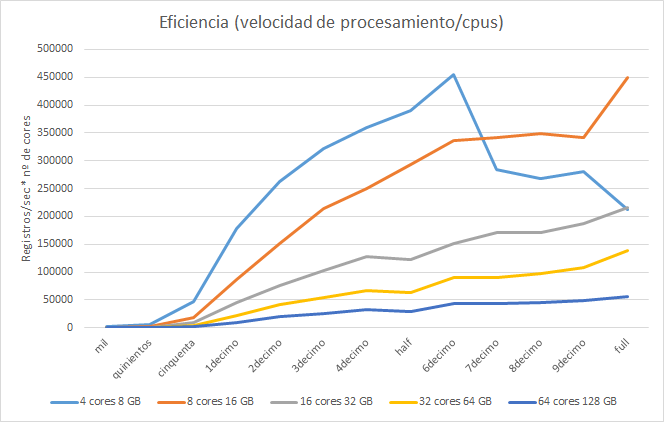
\includegraphics[scale=0.8]{graficas/ebuni}
\end{figure}
\begin{figure}[htp!]
	\centering
	\caption{Gráfica comparativa de la eficiencia durante la consulta de zonas que reportan más beneficio teniendo en cuenta la estacionalidad por el clúster universitario.}
	\label{gra:efiProDayUniApen}
	\vspace{5pt}
	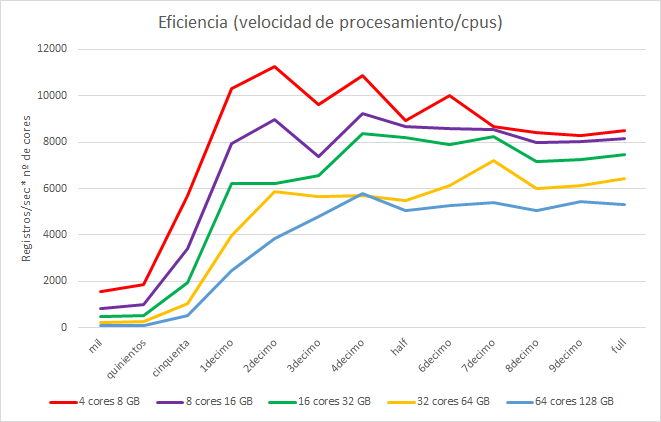
\includegraphics[scale=0.8]{graficas/ebduni}
\end{figure}

\chapter{Fichero ``slaves'' para las diferentes configuraciones del clúster universitario \label{slavesUni}}
\begin{lstlisting}[label=2nodos,language=C,frame=single,caption=Fichero ``slaves'' para configuración con dos nodos]
lm001.lab.it.uc3m.es
lm002.lab.it.uc3m.es
\end{lstlisting}
\begin{lstlisting}[label=4nodos,language=C,frame=single,caption=Fichero ``slaves'' para configuración con cuatro nodos]
lm001.lab.it.uc3m.es
lm002.lab.it.uc3m.es
lm003.lab.it.uc3m.es
lm004.lab.it.uc3m.es
\end{lstlisting}
\begin{lstlisting}[label=8nodos,language=C,frame=single,caption=Fichero ``slaves'' para configuración con ocho nodos]
lm001.lab.it.uc3m.es
lm002.lab.it.uc3m.es
lm003.lab.it.uc3m.es
lm004.lab.it.uc3m.es
lm005.lab.it.uc3m.es
lm006.lab.it.uc3m.es
lm007.lab.it.uc3m.es
lm008.lab.it.uc3m.es
\end{lstlisting}
\clearpage
\begin{lstlisting}[label=16nodos,language=C,frame=single,caption=Fichero ``slaves'' para configuración con dieciseis nodos]
lm001.lab.it.uc3m.es
lm002.lab.it.uc3m.es
lm003.lab.it.uc3m.es
lm004.lab.it.uc3m.es
lm005.lab.it.uc3m.es
lm006.lab.it.uc3m.es
lm007.lab.it.uc3m.es
lm008.lab.it.uc3m.es
lm009.lab.it.uc3m.es
lm010.lab.it.uc3m.es
it002.lab.it.uc3m.es
it003.lab.it.uc3m.es
it004.lab.it.uc3m.es
it005.lab.it.uc3m.es
it006.lab.it.uc3m.es
it007.lab.it.uc3m.es
\end{lstlisting}


\chapter{Sistema de celdas del mapa \label{cuadricula}}
\section{Características}
Las características del mapa de la ciudad y de las cuadrículas son las siguientes:

\begin{itemize}
\item El mapa está compuesto de 300 cuadrículas de alto por 300 de ancho (300x300).
\item Cada cuadrícula corresponde a 0,5 km de ancho y de alto. Esto corresponde a 0,004491556 en latitud y 0,005986 en longitud.
\item La cuadrícula del mapa empieza en la celda (1,1) cuyo centro se sitúa en la posición 41.474937 de latitud y -74.913585 de longitud, que se encuentra en Barryville. (41.474937, -74.913585)
\item Los números de las celdas se expanden hacia el este y el sur, donde el este es la primer componente de la posición y, el sur, la segunda. \textbf{Posición -> (X,Y) donde X = Este, Y = Sur}
\item El mapa se expandirá 150 kilómetros al este y sur, suponiendo la celda (300,300) la máxima amplitud.
\item No se tendrán en cuenta los viajes que empiecen o terminen fuera de las celdas indexadas.
\end{itemize}


\section{Tratamiento de las celdas}

El mapa lo guardaremos en una lista que contendrá la información de cada cuadrícula del mapa. Esta información consistirá en una tupla que contendrá los siguientes datos:

\begin{itemize}
\item Coordenadas de la casilla. (X,Y).
\item Posición esquina superior izquierda (latitud, longitud).
\end{itemize}

Estos datos serán inmutables y, por razones de velocidad de acceso, serán guardados en tuplas de Python.

\section{Primera celda}

Como se ha indicado anteriormente, la primera celda (1,1) tiene el punto central en las coordenadas (41.474937, -74.913585), por lo que hay que calcular la posición de la esquina superior izquierda de esta primera para posteriormente calcular la posición del resto de las cuadrículas del mapa. Por tanto:

\begin{itemize}
\item Latitud de la esquina superior izquierda -> 41.474937 + 0,004491556/2 = 41.477182778.
\item Longitud esquina superior izquierda -> -74.913585 - 0.005986/2 = -74.916578
\end{itemize}
    
La posición de la esquina superior de la cuadrícula (1,1) es (41.477182778,-74.916578). Por tanto, cada cuadrícula tendrá la siguiente forma:

\begin{verbatim}
punto = (X, Y, latitudEsqIzqSup, longitudEsqIzqSup)
\end{verbatim}

\begin{lstlisting}[label=cuadriculaCSV,language=Python,frame=single,caption=Código para crear fichero con las coordenadas de cada cuadrícula]
from settings import *
import numpy as np
import pandas as pd

p = (1, 1, 41.477182778, -74.916578)
mapa = []
for y in range(MAPSIZE):
    for x in range(MAPSIZE):
        mapa.append((p[0]+x, p[1]+y, p[2]-(y*LATITUDE), p[3]+(x*LONGITUDE)))
fichero = pd.DataFrame(data=mapa,columns=["X", "Y", "LATITUD", "LONGITUD"])
fichero.to_csv("CuadriculaMapa.csv")
\end{lstlisting}

El código para crear un fichero \gls{CSV} con el índice de cuadrículas y sus coordenadas se puede encontrar en el fragmento \ref{cuadriculaCSV}.